\documentclass{standalone}
\usepackage{pgfplots}
\pgfplotsset{compat=newest}

\begin{document}
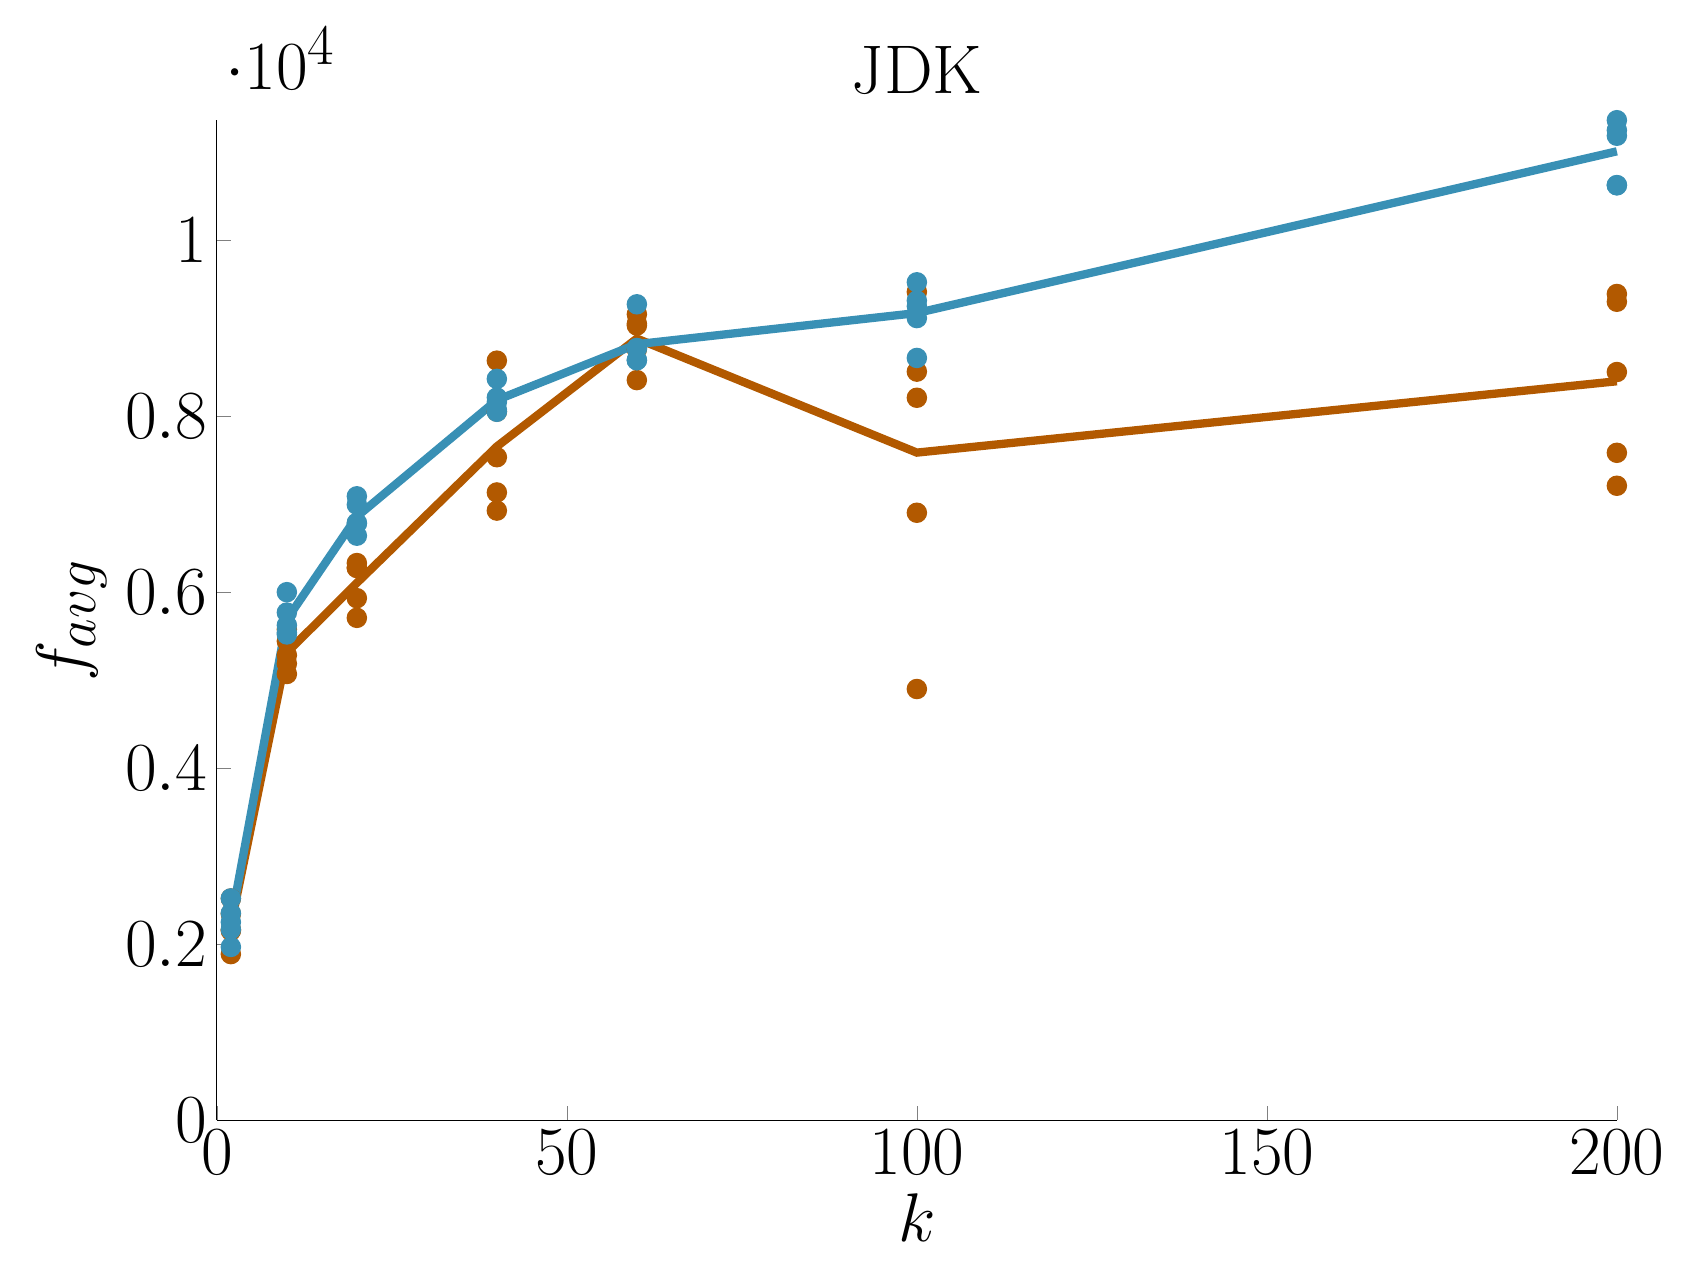
\begin{tikzpicture}

\begin{axis}[%
title style={font=\Huge},
title=JDK,
tick label style={font=\Huge},
label style={font=\Huge},
legend style={font=\Huge},
view={0}{90},
max space between ticks=50pt,
width=7in,
height=5in,
scale only axis,
xmin=0, xmax=200,
xtick={0, 50, 100, 150, 200},
xlabel={$k$},
ymin=0, ymax=11364.8,
%ytick={0, 200, 400, 600, 800, 1000},
ylabel={$f_{avg}$},
major tick length=5pt,
axis lines*=left,
legend cell align=left,
clip=false]

\addplot [
only marks,
mark=*,
mark size=3.5pt,
color=orange!70!black,
%solid,
%line width=2pt,
]
coordinates{
(2,1887.6)(2,2152.9)(2,2164.55)(2,2345.35)(2,2519.6)(10,5071.15)(10,5189.05)(10,5284.5)(10,5443.9)(10,5578.35)(20,5709.2)(20,5932.85)(20,6275.95)(20,6279.2)(20,6331.8)(40,6928.05)(40,7134.2)(40,7534.95)(40,8053.3)(40,8632.35)(60,8411.35)(60,8761.55)(60,9031.65)(60,9051.6)(60,9159.05)(100,4900.45)(100,6903.6)(100,8210.45)(100,8507.35)(100,9413.95)(200,7210.5)(200,7584.9)(200,8502.95)(200,9301.45)(200,9389.7)
};

\addplot [
only marks,
mark=*,
mark size=3.5pt,
color=cyan!70!black,
%solid,
%line width=2pt,
]
coordinates{
(2,1968.8)(2,2167.55)(2,2250.8)(2,2353.45)(2,2520.55)(10,5520.65)(10,5540.15)(10,5625.2)(10,5769.75)(10,6001.05)(20,6642.55)(20,6781.05)(20,6789.25)(20,6995.15)(20,7090.65)(40,8051.0)(40,8072.15)(40,8161.65)(40,8212.85)(40,8425.2)(60,8637.3)(60,8637.85)(60,8774.15)(60,8774.95)(60,9272.65)(100,8662.95)(100,9116.0)(100,9250.35)(100,9314.7)(100,9522.6)(200,10624.45)(200,10627.5)(200,11187.95)(200,11250.7)(200,11364.8)
};

\addplot [
color=orange!70!black,
solid,
line width=3pt
]
coordinates{
(2,2214.0)(10,5313.39)(20,6105.8)(40,7656.57)(60,8883.04)(100,7587.16)(200,8397.9)
};

\addplot [
color=cyan!70!black,
solid,
line width=3pt
]
coordinates{
(2,2252.23)(10,5691.36)(20,6859.73)(40,8184.57)(60,8819.38)(100,9173.32)(200,11011.08)
};


\end{axis}
\end{tikzpicture}
\end{document}
